\chapter{Concurrency}

\section{The Foundations of Concurrency in Rust}

Concurrency is the art of structuring a program so that multiple tasks can be executed independently, potentially overlapping in time. While \textit{parallelism} refers to the simultaneous execution of tasks (typically across multiple CPU cores), \textit{concurrency} is a broader concept that focuses on managing multiple interleaved execution streams.

In traditional programming languages, shared-state concurrency is notoriously difficult. Data races, where two or more threads access a shared memory location concurrently (with at least one performing a write), lead to Undefined Behavior (UB) and subtle, hard-to-reproduce bugs. 

Rust takes a radically different approach to concurrency. By leveraging the ownership model, borrowing rules, and the type system, Rust eliminates data races at compile time. This principle is famously known as \textbf{"Fearless Concurrency"}.

\begin{insightbox}
\textbf{Data Races vs. Race Conditions} \\
Safe Rust strictly prevents \textit{data races} (concurrent read/write without synchronization). However, Rust does \textit{not} prevent general \textit{race conditions} (where the timing of thread execution affects the program's logical outcome), nor does it prevent deadlocks. Logic bugs can still occur, but memory unsafety is eliminated.
\end{insightbox}

\section{Creating and Managing Threads}

In Rust, the operating system manages threads natively. You can spawn a new native thread using the \texttt{std::thread::spawn} function. This function takes a closure containing the code that the new thread will execute.

\begin{lstlisting}[language=Rust]
use std::thread;
use std::time::Duration;

fn main() {
    let handle = thread::spawn(|| {
        for i in 1..=5 {
            println!("Hello from the spawned thread: {}", i);
            thread::sleep(Duration::from_millis(1));
        }
    });

    for i in 1..=5 {
        println!("Hello from the main thread: {}", i);
        thread::sleep(Duration::from_millis(1));
    }

    // Wait for the spawned thread to finish
    handle.join().unwrap();
}
\end{lstlisting}

When \texttt{thread::spawn} is called, it returns a \texttt{JoinHandle}. The main thread can call the \texttt{join} method on this handle to block its own execution until the spawned thread terminates. Without calling \texttt{join}, the spawned thread might be forcefully terminated if the main thread completes its execution first.

\subsection{Capturing Environment with \texttt{move}}

Often, a thread needs to access variables defined in the environment that spawned it. By default, closures capture variables by reference. However, the Rust compiler cannot guarantee how long a spawned thread will live; it might outlive the environment that created the variables!

To solve this, we use the \texttt{move} keyword to force the closure to take \textbf{ownership} of the variables it captures.

\begin{lstlisting}[language=Rust]
use std::thread;

fn main() {
    let v = vec![1, 2, 3];

    let handle = thread::spawn(move || {
        println!("Here's a vector: {:?}", v);
    });

    handle.join().unwrap();
}
\end{lstlisting}

\begin{warningbox}
\textbf{The Missing \texttt{move}} \\
Forgetting the \texttt{move} keyword when trying to use external variables in a \texttt{thread::spawn} closure is one of the most common compile-time errors for beginners. The compiler will complain that the borrowed value may not live long enough, safely catching a potential dangling pointer.
\end{warningbox}

\section{The Safety Net: \texttt{Send} and \texttt{Sync} Traits}

Rust's concurrency guarantees are grounded in two special traits: \texttt{Send} and \texttt{Sync}. These are \textit{marker traits}, meaning they have no methods. They exist solely to inform the compiler about the concurrency properties of a type.

\begin{itemize}
    \item \textbf{\texttt{Send}} indicates that ownership of a value of this type can be transferred safely between threads. Almost all Rust types are \texttt{Send}. A notable exception is \texttt{Rc<T>}, the reference-counted smart pointer, which is not thread-safe.
    \item \textbf{\texttt{Sync}} indicates that it is safe for a type to be referenced from multiple threads. Formally, a type \texttt{T} is \texttt{Sync} if \texttt{\&T} (an immutable reference to \texttt{T}) is \texttt{Send}.
\end{itemize}

The compiler automatically implements these traits for composite types if all their members implement them. You rarely need to implement \texttt{Send} or \texttt{Sync} manually, and doing so requires the \texttt{unsafe} keyword.

\begin{exambox}
\textbf{Exam Focus: Identifying \texttt{Send}/\texttt{Sync} Violations} \\
Exam questions frequently ask you to spot why a specific snippet of concurrent code fails to compile. Look out for types like \texttt{Rc<T>} or \texttt{RefCell<T>} being passed across thread boundaries. Since they do not implement \texttt{Send} and \texttt{Sync}, the compiler will reject the code. The correct thread-safe alternatives are \texttt{Arc<T>} and \texttt{Mutex<T>}.
\end{exambox}

\section{Shared-State Concurrency}

While message passing (discussed next) is a popular concurrency model, sharing memory is sometimes necessary. The core tool for safe shared memory in Rust is the \texttt{Mutex} (Mutual Exclusion).

\subsection{Protecting Data with \texttt{Mutex}}

A \texttt{Mutex} encapsulates data, requiring threads to explicitly acquire a lock before they can access it. This ensures that only one thread can access the data at any given time, preventing data races.

\begin{lstlisting}[language=Rust]
use std::sync::Mutex;

fn main() {
    let m = Mutex::new(5);

    {
        // Acquire the lock. It blocks if another thread holds the lock.
        let mut num = m.lock().unwrap();
        *num = 6;
        // The lock is automatically released when `num` goes out of scope.
    }

    println!("m = {:?}", m);
}
\end{lstlisting}

Calling \texttt{lock()} returns a \texttt{MutexGuard}, a smart pointer that provides mutable access to the underlying data. The lock is automatically released (via the \texttt{Drop} trait) when the \texttt{MutexGuard} goes out of scope.

\begin{notebox}
\textbf{Poisoned Mutexes} \\
Notice the \texttt{.unwrap()} after \texttt{lock()}. If a thread panics while holding a mutex lock, the mutex becomes \textit{poisoned}. Future attempts by other threads to lock it will result in an \texttt{Err}, ensuring that threads don't accidentally observe data in an inconsistent state.
\end{notebox}

\subsection{Sharing Mutexes with \texttt{Arc}}

To share a \texttt{Mutex} across multiple threads, we need multiple owners. In a single-threaded context, we use \texttt{Rc<T>}. In a concurrent context, we must use \textbf{\texttt{Arc<T>}} (Atomic Reference Counted). \texttt{Arc} ensures that the reference count is incremented and decremented atomically, making it safe to share across threads.

\begin{lstlisting}[language=Rust]
use std::sync::{Arc, Mutex};
use std::thread;

fn main() {
    // Arc allows multiple ownership, Mutex allows interior mutability.
    let counter = Arc::new(Mutex::new(0));
    let mut handles = vec![];

    for _ in 0..10 {
        let counter_clone = Arc::clone(&counter);
        let handle = thread::spawn(move || {
            let mut num = counter_clone.lock().unwrap();
            *num += 1;
        });
        handles.push(handle);
    }

    for handle in handles {
        handle.join().unwrap();
    }

    println!("Result: {}", *counter.lock().unwrap()); // Prints 10
}
\end{lstlisting}

\section{Message Passing with \texttt{mpsc}}

An increasingly popular approach to concurrency, heavily inspired by languages like Go, is \textbf{message passing}. The guiding principle is: \textit{"Do not communicate by sharing memory; instead, share memory by communicating."}

Rust's standard library provides channels for message passing via the \texttt{std::sync::mpsc} module. \textbf{mpsc} stands for \textbf{Multiple Producer, Single Consumer}.

\begin{figure}[h]
    \centering
    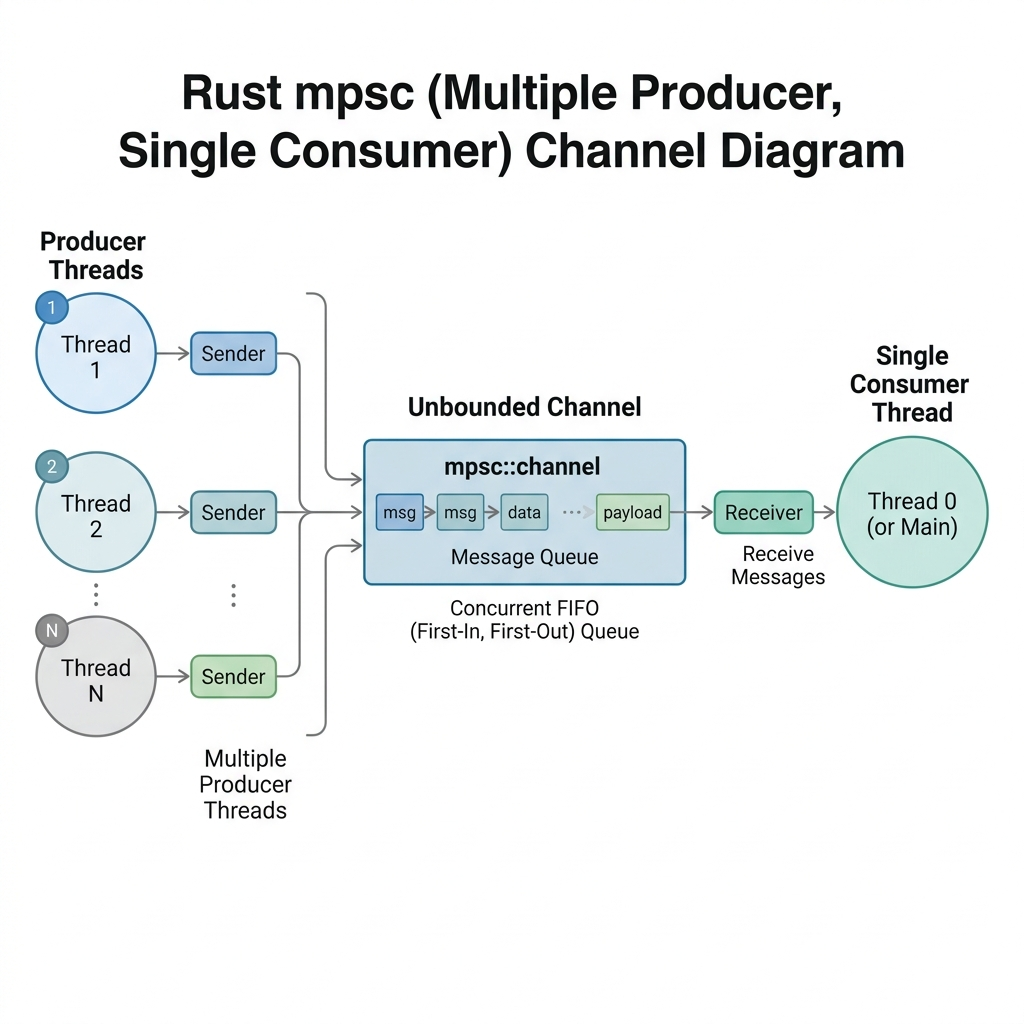
\includegraphics[width=\textwidth]{images/mpsc_channel.png}
    \caption{Architecture of a Multiple Producer, Single Consumer (MPSC) channel.}
    \label{fig:mpsc}
\end{figure}

A channel consists of two halves: a transmitter (\texttt{Sender}) and a receiver (\texttt{Receiver}).
You can clone the \texttt{Sender} to create multiple producers, but there can only be one \texttt{Receiver}.

\begin{lstlisting}[language=Rust]
use std::sync::mpsc;
use std::thread;
use std::time::Duration;

fn main() {
    let (tx, rx) = mpsc::channel();
    
    // Clone the transmitter for a second thread
    let tx1 = tx.clone();

    thread::spawn(move || {
        let vals = vec![
            String::from("hi"),
            String::from("from"),
            String::from("thread 1"),
        ];
        for val in vals {
            tx1.send(val).unwrap();
            thread::sleep(Duration::from_millis(200));
        }
    });

    thread::spawn(move || {
        let vals = vec![
            String::from("more"),
            String::from("messages"),
            String::from("for you"),
        ];
        for val in vals {
            tx.send(val).unwrap();
            thread::sleep(Duration::from_millis(200));
        }
    });

    // The receiver acts as an iterator that blocks until messages arrive.
    for received in rx {
        println!("Got: {}", received);
    }
}
\end{lstlisting}

When you call \texttt{send}, it takes ownership of the value and moves it to the receiver. This prevents the producer from accidentally modifying the message after sending it, preserving memory safety. The \texttt{Receiver} implements the \texttt{Iterator} trait, which blocks waiting for new messages. The loop automatically terminates when all \texttt{Sender} instances have been dropped, as this signals that no more messages will ever be sent.

\begin{insightbox}
\textbf{Channels vs. Shared State} \\
Channels simplify complex synchronization scenarios by creating clear, unidirectional data flows. Shared state (via \texttt{Arc<Mutex<T>>}) is better suited when multiple threads need continuous read/write access to a complex, monolithic data structure.
\end{insightbox}

\section*{End-of-Chapter Exam Questions}

\begin{enumerate}
    \item \textbf{Conceptual (Traits):} A developer is attempting to pass a structure \texttt{Config} containing a \texttt{Rc<String>} across a thread boundary using \texttt{thread::spawn}. The compiler rejects the code. Explain why this happens referencing the \texttt{Send} and \texttt{Sync} traits, and propose a solution that satisfies the compiler while maintaining the original semantic intent.
    
    \item \textbf{Conceptual (Channels):} Describe the \texttt{mpsc} model. Why does the standard library provide a `Multiple Producer, Single Consumer` primitive rather than a `Multiple Producer, Multiple Consumer` (mpmc) one? What happens to the \texttt{Receiver} iterator when the last cloned \texttt{Sender} goes out of scope?
    
    \item \textbf{Coding (Shared State):} You are given an \texttt{Arc<Mutex<Vec<i32>>>}. Write a short Rust snippet that spawns 4 threads. Each thread should push its own thread ID (0, 1, 2, or 3) into the shared vector 5 times. Ensure the main thread waits for all spawned threads to complete before printing the final length of the vector.
\end{enumerate}
